\section{Methodology}
The 2023 iteration of the CaveX project builds upon the existing work using robust project management strategies to ensure its objectives are achieved. A systems engineering approach is utilised to facilitate such accomplishments. Applying the systems engineering practices ensures that the engineering process is strictly informed by stakeholder needs. The stakeholder needs have been carried through both the 2021 and 2022 iterations of the CaveX project and have been adjusted according to stakeholder meetings. Periodic communication with the primary stakeholders ensures that the team is building the right system to meet stakeholder expectations which will ensure the system can successfully be validated. The implementation of the project objective's are to be done using an agile software engineering approach to allow for tasks to be completed in parallel.

\subsection{Systems Engineering}
The 2023 CaveX team will follow a systems engineering approach, shown in Figure \ref{fig:systemsVdiagram}, to fully break down and define the problem at hand and develop an innovative solution that meets the expectations of the final user.

\begin{figure}[H]
    \centering
    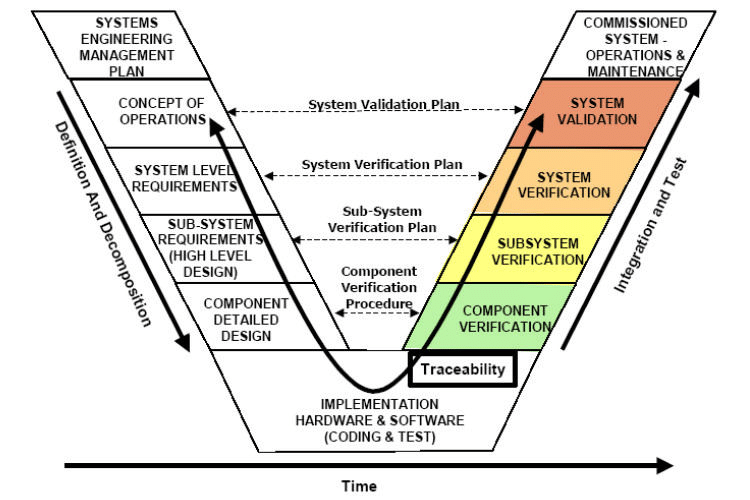
\includegraphics[scale=0.5]{images/The-Systems-Engineering-V-Diagram.png}
    \caption{The Systems Engineering "V" Diagram (Allouis et al. 2013)}
    \label{fig:systemsVdiagram}
\end{figure}

The problem definition phase at the beginning of the systems engineering "V" diagram will consist of a detailed stakeholder analysis to identify and understand all of the groups that can affect the project or are directly affected by the project. A stakeholder analysis is also important to understand potential restrictions from stakeholders and defines which groups of people should be closely worked with throughout the duration of the project. To better understand the entities that the system is interacting with a system context analysis will be conducted. The context of the system will assist in defining interface requirements for external systems that the CaveX robot will interact with.

The next important phase of the systems engineering approach is requirements development. In this stage of the design process it is essential to understand the needs of the final user which will be transformed into system level requirements that guide the technical design. This project builds upon the user needs that were identified in the previous design iterations with slight adjustments due to discussions with primary stakeholders that focus on the autonomous direction of the project. A useful tool in understanding the fundamental needs of the user is to conduct a scenario based needs analysis where a typical use of the robotic system and all of the functions that are necessary to achieve the desired mission is analysed. After the user needs are identified system requirements which define functional and non-functional specifications for the final design are developed. The system requirements are developed in a similar way to the SMART framework used to describe the technical objectives in Appendix \ref{app:smartobj}. In particular, the requirements should be measurable to assist in the verification of the final design towards the end of the project.

After the development of system requirements a functional analysis will be conducted and concept solutions will be explored. The functional analysis will divide the system into smaller functional elements which assists in understanding key functionality and subsystem requirements. A literature review is essential to identify solutions to similar problems and how they could be applicable to this problem. In the literature review a range of different algorithms for autonomous functionality must be explored to understand the advantages and disadvantages of each approach. After a range of different algorithms are explored a preliminary concept design will be presented.

Verification and validation occurs towards the end of the engineering process. Full system validation is to be done at the Naracoorte Caves with the primary user Craig Williams to demonstrate the system has the required functionality to meet the needs of a user. The verification process involves ensuring the system has been built correctly and meets the technical objectives. Each of the system requirements listed in Table \ref{tab:sysreq} will be verified at the end of the project. There are four primary methods of verification which include analysis, inspection, demonstration, and testing. Demonstration and testing are the most costly but have the highest confidence in successfully assessing the quality of the final design. Inspection and analysis verification methods are of low confidence and should only be used in verification when it is infeasible to extensively test the system. To ensure a high level of quality, each system requirement will either be tested or the required functionality will be demonstrated. As outlined in the quality assurance plan in Appendix \ref{app:qualityplan}, unit tests will be performed throughout the implementation phase to eliminate bugs early in the design process.

\subsection{Agile Engineering}
\label{agile_software_engineering}
The implementation of the project's objectives is managed using an agile engineering methodology. This approach suits the project well, being a predominantly software-oriented project. The agile approach applied to software development allows for faster responses to changing requirements and situations which may present themselves during the project's duration. To compliment the agile software engineering approach, organised software development sprints have been devised. A plan for these sprints is shown in the Appendix \ref{app:sprintplan} and a schedule is shown in the Gantt chart in Appendix \ref{app:ganttChart}. Some of the technical objectives in Table \ref{tab:objectives} are independent of others and, therefore, allows objective sub-tasks to be managed in a flexible manner. Hence, for an agile approach there is no definitive plan for the work to be be conducted in each sprint. Deadlines have been set for technical objective completion to provide an approximate timeline for task completion. These deadlines are also shown in the Gantt chart. 

Jira is an issue tracking software developed by Atlassian that is utilised by many software engineering teams to manage workloads. It is used to assist the team in breaking down work into smaller tasks that can be assigned to individual group members. A snapshot of the 2023 Jira task board is shown in Figure \ref{fig:jira_taskboard}.

\begin{figure}[H]
    \centering
    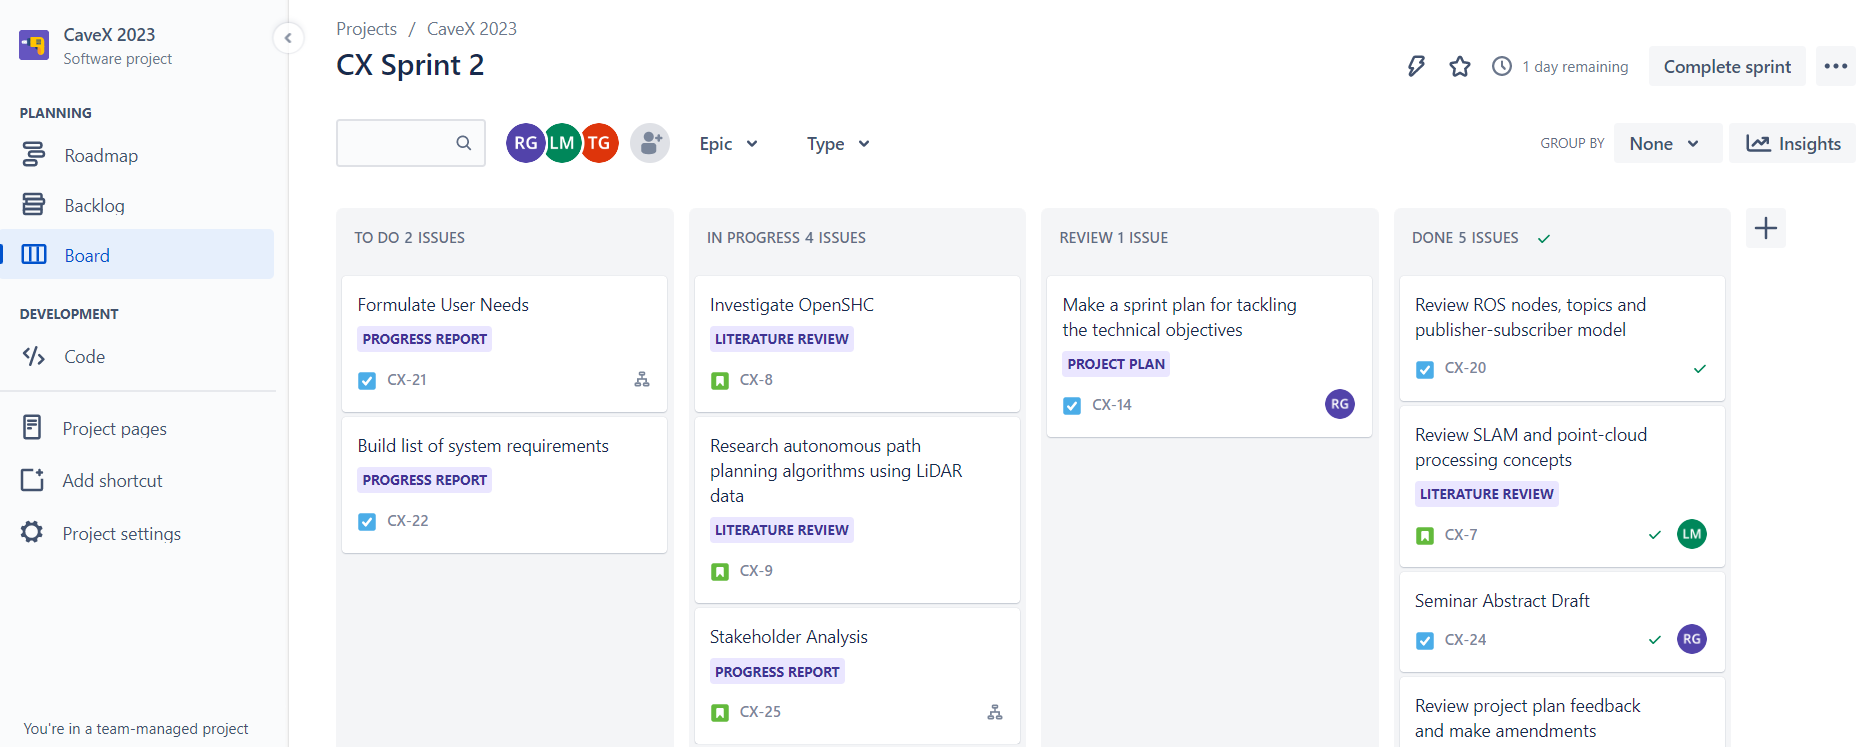
\includegraphics[scale=0.4]{images/jira taskboard.png}
    \caption{Snapshot of the Jira taskboard used for project management}
    \label{fig:jira_taskboard}
\end{figure}

Managing tasks using Jira has many benefits including a focus on project schedule and scope management. Therefore, using Jira allows for consistency with the work breakdown structure shown in Appendix \ref{app:WBS} and the project Gantt chart. Jira allows for tasks to be added to specific iterations of the software implementation which are the software development sprints. The sprints are four weeks in length and an approximate sprint plan is shown in Appendix \ref{app:sprintplan}. This plan is used to manage the schedule of the project to ensure the objectives are completed by their deadlines. It is consistent with the schedule in the Gantt chart and the estimated objective completion dates stated in section \ref{aims_scope_objectives}. Where possible, objectives are designed such that they can be developed in parallel to mitigate the risk of unforeseen delays in early implementations which could be carried down the project timeline. These risks are prominent with a waterfall software engineering approach where functionality is implemented incrementally and depends heavily on predecessor milestones being completed. Hence, an agile methodology is justified to give the team flexibility in the schedule to investigate different functionality as it becomes necessary.